101. \begin{figure}[ht!]
\center{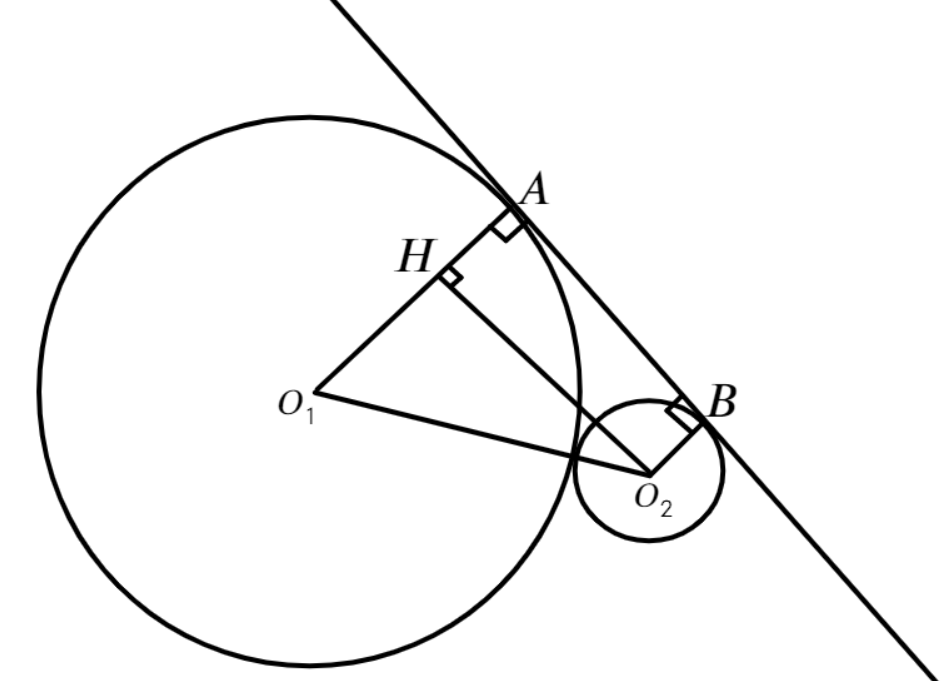
\includegraphics[scale=0.35]{g8-102.png}}
\end{figure}\\
Соединим центры окружностей друг с другом и с точками касания. Так как центры окружностей лежат на одной прямой с точкой касания, а радиусы перпендикулярны касательной, $AO_1O_2B$ --- прямоугольная трапеция, в которой $AO_1=4R,\ BO_2=R,\ O_1O_2=4R+R=5R,\ AB=8$см. Опустим высоту $O_2H,$ тогда $O_1H=4R-R=3R,$ а $O_2H=AB=8$см. По теореме Пифагора для треугольника $O_1HO_2$ имеем $25R^2=9R^2+64,\ R^2=4,\ R=2$см. Значит, радиусы окружностей равны 2 см и $2\cdot4=8$см.\\
